 \label{relationMoyDHmoyDC}
 
Nous allons calculer les corr\'elations entre les distances de correction et de Hamming en se basant sur le  graphe $G$, son line-graphe $LG$ et le line-graphe $LG_{k,p, \alpha}$ obtenu par notre couple d'algorithmes.
Notre objectif est de montrer la relation entre ces deux distances.
\newline
Consid\'erons les distances de correction et de Hamming obtenues par l'approche {\em al\'eatoire sans remise}, la variable $p = 0.5$ et la fonction de co\^ut {\em unitaire} (voir tableau \ref{tab:recapApprocheCorrection}).

% ----------------------------- figure  correlation distance hamming distance correlation -------------------- 
 \begin{figure}[htb!] 
\centering
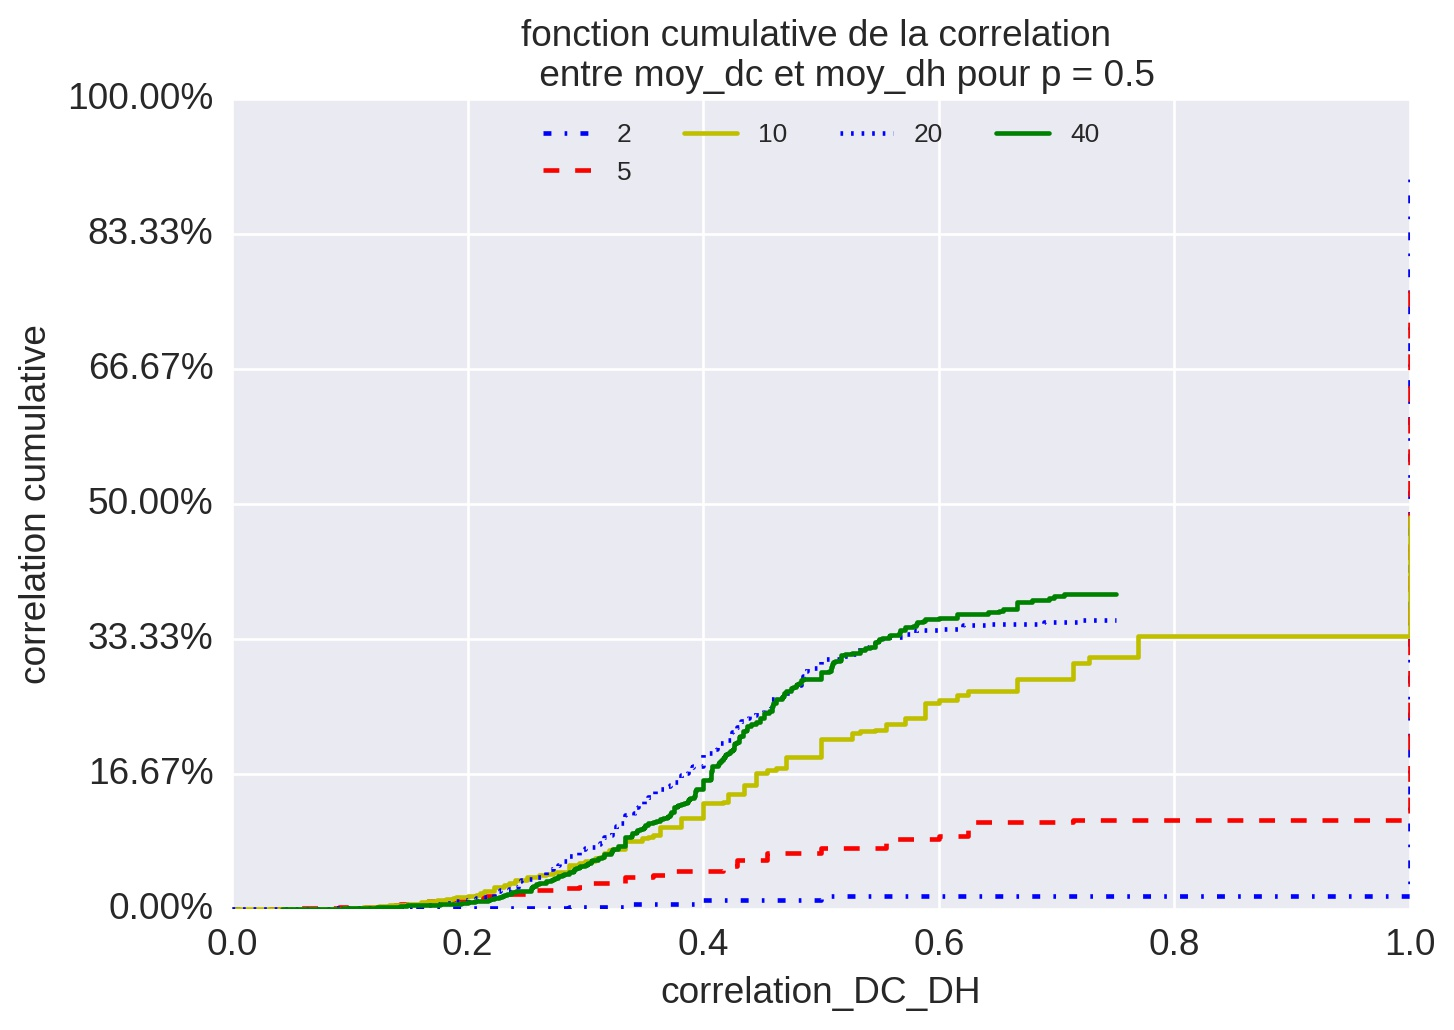
\includegraphics[scale=0.35]{correlation_dh_dl_p_05.jpeg}
\caption{ La corr\'elation de la distance de correction versus la distance de Hamming pour $k$ cases modifi\'ees et $p = 0.5$ }
\label{dh_vs_dc_p_05} 
\end{figure}
\FloatBarrier
% ----------------------------- figure  correlation distance hamming distance correlation -------------------- 

Nous calculons la corr\'elation entre les distances de correction et de Hamming avec la formule \ref{correlation_correction_hamming}.
%\begin{multline}
\begin{equation}
	corr_{k,p,\alpha} =  \frac{ | moy\_DC_{k, p,\alpha} - moy\_DH_{k,p, \alpha} | }{ max(moy\_DC_{k, p,\alpha},  moy\_DH_{k, p, \alpha}) };
	\\
	corr_{k,p} = \sum_{\alpha = 1}^{5}corr_{k,p,\alpha} ;
	\\ \newline
	F_k (x,p) = P(corr_{k,p} < x ) 
\label{correlation_correction_hamming}
\end{equation}
%\end{multline}
avec $x \in [0,1]$ une valeur de corr\'elation et $k$ le nombre de cases modifi\'ees. 
La fonction $corr_{k,p,\alpha}$ retourne l'\'ecart entre ces deux distances sous la forme de valeurs probabilistes. 
Ainsi $corr_{k,p,\alpha} = 1$ indique qu'il n'existe aucune corr\'elation entre les distances de correction et de Hamming c'est-\`a-dire que $moy\_DC_{k,p,\alpha} = k$ et $moy\_DH_{k,p,\alpha} = 0$.
De m\^eme, $corr_{k,p} = 0$ indique que ces distances sont identiques c'est-\`a-dire $ moy\_DC_{k, p, \alpha} = moy\_DH_{k,p, \alpha}$. En moyenne, $moy\_DH_{k,p, \alpha}$ tend vers $k$ cases modifi\'ees. 
\newline

La figure \ref{dh_vs_dc_p_05} repr\'esente la fonction de repartition $F_k$ dans laquelle nous avons, en abscisse, la corr\'elation entre les distances et, en ordonn\'e, le pourcentage de graphes dont la corr\'elation moyenne $corr_{k,p}$ est inf\'erieure \`a $x \in [0,1]$. 
%si $F_k$ a une courbe d'\'equation $y = 100$  ====> intuition pour la definition F_k
Si $corr_{k,p,\alpha} = 0$ alors les matrices de $LG_{k,p,\alpha}$ et $LG$ sont diff\'erentes de $k$ cases quand $k < 6$ ($LG_{k,p,\alpha} \neq LG$).
Si $corr_{k,p,\alpha} = 1$ alors le line-graphe $LG_{k, p, \alpha}$ est le line-graphe du graphe $G$ ($LG_{k, p, \alpha} = LG$) et $F_k(1) \approx 0$. 
La corr\'elation $corr_{k,p} = 1$ est sa valeur maximale. 
Ce cas est illustr\'e dans la figure \ref{dh_vs_dc_p_05} par les courbes de $k \in \{2,5\}$. 
Par exemple $F_5(1) \approx 10\%$ signifie que nous avons $70-10=60\%$ des line-graphes $LG_k$ qui ont le m\^eme ensemble d'ar\^etes que les line-graphes $LG$ ($70\%$ est le pourcentage de corr\'elations \'egales \`a $1$ $|corr_{5,p} = 1 | = 70\%$ ).
\newline
En revanche, une valeur de $F_k(1)$ tr\`es \'elev\'ee signifie que le nombre $x$ de  $corr_{k,p} = 1$ est tr\`es faible. Ce nombre $x$ implique une corr\'elation tr\`es forte entre les distances de correction et de Hamming.
C'est l'observation faite avec les courbes de $k \in \{10,20,40\}$ de la figure \ref{dh_vs_dc_p_05} dans lesquelles nous avons une  croissance continue en fonction de l'augmentation des valeurs de corr\'elations.
\newline
Nous subdivisons nos courbes en deux cat\'egories:
\begin{itemize}
	\item Celles pour lesquelles il y'a une corr\'elation entre les distances de correction et de Hamming (courbes de $k \in \{10,20,40\}$).
	\item Celles pour lesquelles il y'a  aucune corr\'elation entre ces distances parce que   $LG = LG_{k,p}$ (courbes de $k \in \{2,5\}$). 
\end{itemize}


{\bf Conclusion} :
il existe de fortes corr\'elations entre les distances de correction et de Hamming lorsque $k \ge 10$. Dans ce cas, nous pouvons utiliser la distance de correction pour calculer les \'ecarts de cases modifi\'ees pendant l'algorithme de correction.
Dans le cas o\`u $k \le 5$, les distances de correction inf\'erieures ou \'egales \`a $5$ cases proposent le line-graphe $LG$ et ces distance entrainent une corr\'elation proche de $0$.
Pour  $k \in \{6,7,8,9\}$, les valeurs de $corr_{k,p}$ avoisinent $0.5$. Ces valeurs sont faibles et nous ne pouvons rien conclure.
Ainsi, pour juger de la qualit\'e de notre algorithme de correction en l'absence de la distance de Hamming, la distance de correction est alors une bonne m\'etrique.
